\section{Ethan}

\subsection{Aufgabenstellung}

\begin{enumerate}
    \item Energie in Abhängigkeit des Diederwinkels zeichnen und die Anzahl der Min- bzw. Maxima bestimmen.
    \item Auswertung der erhaltenen Werte.
    \item Statistische Fehlerrechnung
    \item Vergleich der Methoden 
    \item Schwingungsspektrum und Bestzungszahlen bestimmen.
    \item Berechnung der Geschwindigkeitskonstante der Rotation 
\end{enumerate}

\subsection{Diagramm der Rotationsbarrieren}
Da die beiden Kohlenstoffatome nur über ein $\sigma$-Bindung miteinander verbunden sind, können sich beide Enden frei derehen. Dabei sind 
manche Winkel energetisch günstiger als Andere. Dies ist gut zu sehen, wenn Ethan in der Newman-Projektion dargestellt wird.

\begin{figure}[H]
    \centering
    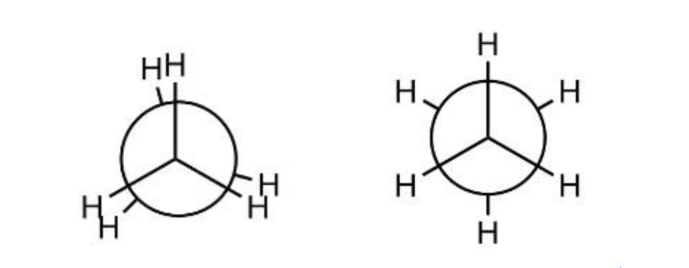
\includegraphics[scale=.7]{../src/img/newmanEthan.png}
    \caption{Newman Darstellung con Ethan}
\end{figure}

Wie man in Abbildung 1 erkennen kann gibt es zwei Extrema, links sind die H-Atome genau hintereinander angeordnet, es kommt somit zu einer größeren
Abstoßung der negativ geladenen $sp^3$-Orbitale. Diese Anordnung nennt sich auch ''eclips''. Bei der rechten Darstellung sind die Orbitale weiter
voneinander entfernt, es können daher nicht zu einer so starke elektrostatischen Abstoßung kommen wie bei der Linken. Diese Anordnung nennt sich ''stacked''.\\
Mit dem Programm HyperChem wurden in der Laboreinheit, die Energieunterschiede zwischen verschieden Diederwinkel bestimmt. Dabei wurden
von jedem Zweierteam sechs semiempirische und zwei ab-initio Methoden verwendet (siehe Abbildung 2 und 3).

\begin{figure}[H]
    \centering
    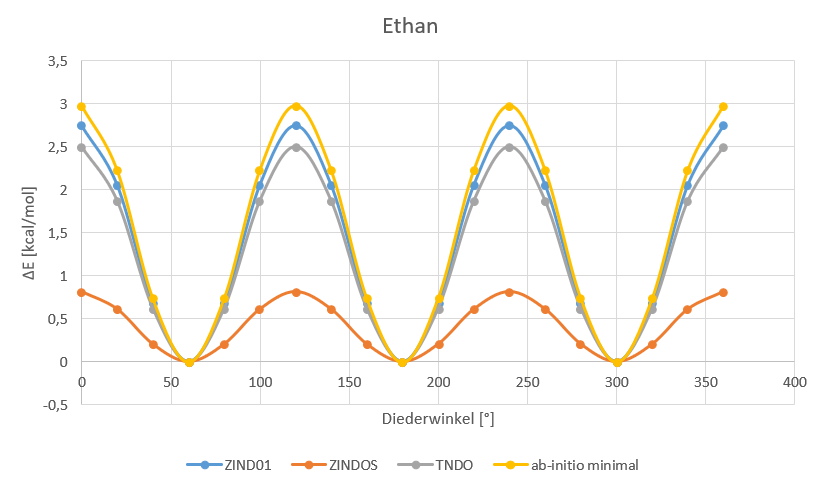
\includegraphics[scale=.7]{../src/img/ethan1.png}
    \caption{Graphische Darstellung der Energiedifferenz gegen den Diederwinkel}
\end{figure}

Um alle Graphen auf eine Achse zu skalieren, wurden von allen, mit HyperChem bestimmten Werte für die elektronische Anregung, die geringste
elektronische Anregung subtrahiert. Dessweiteren sieht man der Graph je vier Maxima und drei Minima bei einer Umdrehung von 360$^\circ$ hat.
Wenn man bei der linken Anordnung aus Abbildung 1 bei $0^\circ$ anfängt, dann sind die Maxima jeweils bei, $0^\circ$, $120^\circ$, $240^\circ$
und wieder bei $360^\circ$. Die Minima befinden sich bei $60^\circ$, $180^\circ$ und $300^\circ$.\\
Weiter ist noch zu sehen, dass alle Methoden verschiedene Ergebnisse liefern, das liegt an der Tatsache, dass jede Methode für eine bestimmte
Aufgabe optimiert wurde und dann andere Parameter nicht berücksichtigt wurden.

\subsection{Auswertung der erhaltenen Werte}
Um den Energieunterschied zwischen der gestaffelten und der verdeckten Konformation zu bestimmen, müssen folgende Werte bekannt sein:
\begin{itemize}
    \item Die maximale und minimale ZPE (Zero Point Energie).
    \item Die maximale und minimale Energie der elektronischen Anregung.
\end{itemize}
Mit diesen Werten kann über folgende Beziehung bestimmt werden:
\begin{align*}
    \Delta \braket{\tilde{e}}(T) &= \Delta e^V (0) + \Delta e^{el} (0) \\
                                 &= \Delta ZPE + \Delta e^{el}   
\end{align*} 
Damit gilt:
\begin{align}
    \Delta e_{mol} = \Delta ZPE + \Delta e^{el} 
\end{align}
% Table generated by Excel2LaTeX from sheet 'Eingabe'
\begin{table}[H]
  \centering
  \caption{Berechnungen der Energien}
  \begin{tabular}{lrrrrrrr}
    \toprule
    \textbf{Methode} & \multicolumn{1}{l}{\boldmath{}\textbf{$e^{el}_{min}$ [kcal/mol]}\unboldmath{}} & \multicolumn{1}{l}{\boldmath{}\textbf{$ZPE_{min}$}\unboldmath{}} & \multicolumn{1}{l}{\boldmath{}\textbf{$e^{el}_{max}$}\unboldmath{}} & \multicolumn{1}{l}{\boldmath{}\textbf{$ZPE_{max}$}\unboldmath{}} & \multicolumn{1}{l}{\boldmath{}\textbf{$\Delta e_{elec}$}\unboldmath{}} & \multicolumn{1}{l}{\boldmath{}\textbf{$\Delta ZPE$}\unboldmath{}} & \multicolumn{1}{l}{\boldmath{}\textbf{$\Delta e_{mol}$}\unboldmath{}} \\
    \midrule
    \textit{ZIND01} & -1821,792 & 65,930 & -1819,042 & 65,245 & 2,749 & -0,685 & 2,064 \\
    \textit{ZINDOS} & -3491,392 & 64,060 & -3490,575 & 62,859 & 0,818 & -1,201 & -0,383 \\
    \textit{TNDO} & -1842,166 & 65,250 & -1839,666 & 64,564 & 2,500 & -0,686 & 1,814 \\
    \textit{ab-initio minimal} & -49137,871 & 56,280 & -49134,887 & 55,622 & 2,984 & -0,658 & 2,326 \\
    \midrule
    \textit{AM1} & -7821,005 & 46,608 & -7819,756 & 46,112 & 1,249 & -0,496 & 0,753 \\
    \textit{RM1} & -7763,136 & 45,194 & -7761,745 & 44,604 & 1,391 & -0,590 & 0,801 \\
    \textit{PM3} & -7611,633 & 46,476 & -7610,204 & 45,845 & 1,429 & -0,631 & 0,798 \\
    \textit{Ab-Initio(Small)} & -49443,952 & 50,230 & -49440,147 & 49,845 & 3,805 & -0,385 & 3,420 \\
    \midrule
    \midrule
    \textit{Mittelwert} &       &       &       &       & 2,116 & -0,666 & 1,449 \\
    \textit{Stabw.} &       &       &       &       & 1,041 & 0,240 & 1,186 \\
    \textit{Präzision MW.} &       &       &       &       & 0,425 & 0,098 & 0,484 \\
    \bottomrule
    \end{tabular}%
  \label{tab:addlabel}%
\end{table}%


\subsection{Statistische Fehlerrechnung}

Um den größtfehler von $\Delta e_{mol} = \Delta ZPE + \Delta e^{el} $ zu bestimmen, wird die Gauß'sche Fehlervorpflanzung benutzt.

\begin{align}
    f(x, y, ...) = \abs{\frac{\delta f}{\delta x}} \cdot \Delta x + \abs{\frac{\delta f}{\delta y}} \cdot \Delta y + ...
\end{align}

Um die Formel besser lesbar zu machen wird $\Delta e_{mol}$ mit f(x, y) ersetzt.

\begin{align*}
    f(x, y) = \abs{\frac{\delt x+y}{\delta x}} \cdot \Delta x + \abs{\frac{\delt x+y}{\delta y}} \cdot \Delta y = \Delta x + \Delta y
\end{align*}

\subsection{Vergleich der Methoden}

\subsection{Schwingungsspektrum und Bestzungszahlen bestimmen}

\subsection{Berechnung der Geschwindigkeitskonstante der Rotation}